\addcontentsline{toc}{chapter}{Appendices}



% The \appendix command resets the chapter counter, and changes the chapter numbering scheme to capital letters.
%\chapter{Appendices}
\appendix
\chapter{Tully Model Paramters}
\label{app:tully_params}

\section{Model 1 -Single Avoided Crossing}
  \begin{minipage}{0.5\textwidth}
      \textbf{Hamiltonian Paramters:}
      \begin{flalign*}
        H_{11}(\mathbf{R}) \ &= \ A \ \tanh(B\mathbf{R}) &\\
        H_{12}(\mathbf{R}) \ &= \ C e^{-D\mathbf{R}^2} \\
        H_{21}(\mathbf{R}) \ &= \ H_{12}(\mathbf{R}) \\
        H_{22}(\mathbf{R}) \ &= \ -H_{11}(\mathbf{R})
      \end{flalign*}
      Where A = 0.03, B = 0.4, C = 0.005 and D = 0.3
  \end{minipage}
  \hspace{0.5cm}
  \vrule
  \hspace{0.5cm}
  \begin{minipage}{0.6\textwidth}
      \begin{tabular}{l|l|c}
        \textbf{Quantity} & \textbf{Value} & \textbf{Unit} \\
        \hline
        Initial Position & -20 & a.u. \\
        Initial Velocities & 15.0, 25.0 & a.u. \\
        Initial Adiab Pop & ground state & - \\
        Simulation Time & 6000, 4000 & a.u. \\
        $\sigma_{\nu}^{(I)}$ & 0.5 & a.u. \\
        M ($\sigma$ constant) & 40 & - \\
        $\Delta t_{\text{nuclear}}$ & 0.1 & fs \\
        $\Delta t_{\text{electonic}}$ & 0.01 & fs \\
        $\frac{\delta \mathbf{R}_{lk, \nu}^{(I)}}{\delta t}$ threshold & 0.15 & a.u. \\
        N$_{rep}$ & 200 & - \\
      \end{tabular}
  \end{minipage}

\section{Model 2 -Dual Avoided Crossing}
\begin{minipage}{0.48\textwidth}
    \textbf{Hamiltonian Paramters:}
    \begin{flalign*}
      H_{11}(\mathbf{R}) \ &= \ 0 &\\
      H_{12}(\mathbf{R}) \ &= \ C e^{-D \mathbf{R}^2} \\
      H_{21}(\mathbf{R}) \ &= \ H_{12}(\mathbf{R}) \\
      H_{22}(\mathbf{R}) \ &= \ -A e^{-B\mathbf{R}^2} + E
    \end{flalign*}
    Where A = 0.1, B = 0.28, C = 0.015, D = 0.06 and E = 0.05
  \end{minipage}
  \hspace{0.5cm}
  \vrule
  \hspace{0.5cm}
  \begin{minipage}{0.6\textwidth}
      \begin{tabular}{l|l|c}
        \textbf{Quantity} & \textbf{Value} & \textbf{Unit} \\
        \hline
        Initial Position & -8 & a.u. \\
        Initial Velocities & 16.0, 30.0 & a.u. \\
        Initial Adiab Pop & ground state & - \\
        Simulation Time & 2500, 1500 & a.u. \\
        $\sigma_{\nu}^{(I)}$ & 0.5 & a.u. \\
        M ($\sigma$ constant) & 40 & - \\
        $\Delta t_{\text{nuclear}}$ & 0.1 & fs \\
        $\Delta t_{\text{electonic}}$ & 0.01 & fs \\
        $\frac{\delta \mathbf{R}_{lk, \nu}^{(I)}}{\delta t}$ threshold & 0.15 & a.u. \\
        N$_{rep}$ & 200 & - \\
      \end{tabular}
  \end{minipage}

\section{Model 3 -Extended Coupling}
\begin{minipage}{0.5\textwidth}
    \textbf{Hamiltonian Paramters:}
    \begin{flalign*}
      H_{11}(\mathbf{R}) \ &= \ A  &\\
      H_{12}(\mathbf{R}) \ &= \ \left \lbrace
      \begin{array}{l}
        B e^{C\mathbf{R}}, \qquad \qquad R \leq 0 \\
          B(2 - e^{-C\mathbf{R}}), \quad R > 0\\
      \end{array} \right . \\
      H_{21}(\mathbf{R}) \ &= \ H_{12}(\mathbf{R}) \\
      H_{22}(\mathbf{R}) \ &= \ -H_{11}(\mathbf{R})
    \end{flalign*}
    Where A = 6$\times$ 10$^{-4}$, B = 0.1 and C = 0.9
  \end{minipage}
  \hspace{0.2cm}
  \vrule
  \hspace{0.6cm}
  \begin{minipage}{0.6\textwidth}
      \begin{tabular}{l|l|c}
        \textbf{Quantity} & \textbf{Value} & \textbf{Unit} \\
        \hline
        Initial Position & -15 & a.u. \\
        Initial Velocities & 10, 30 & a.u. \\
        Initial Adiab Pop & ground state & - \\
        Simulation Time & 5000, 1500 & a.u. \\
        $\sigma_{\nu}^{(I)}$ & 0.5 & a.u. \\
        M ($\sigma$ constant) & 40 & - \\
        $\Delta t_{\text{nuclear}}$ & 0.1 & fs \\
        $\Delta t_{\text{electonic}}$ & 0.01 & fs \\
        $\frac{\delta \mathbf{R}_{lk, \nu}^{(I)}}{\delta t}$ threshold & 0.15 & a.u. \\
        N$_{rep}$ & 200 & - \\
      \end{tabular}
  \end{minipage}


\section{Model 4 -Dual Arch}
\hspace*{-1.5cm}
\begin{minipage}{0.49\textwidth}
    \textbf{Hamiltonian Paramters:}
    \begin{flalign*}
      H_{11}(\mathbf{R}) \ &= \ A  &\\
      H_{12}(\mathbf{R}) \ &= \ \left \lbrace
      \begin{array}{l}
        B \left[ -e^{C(\mathbf{R} - D)} + e^{C(\mathbf{R} + D)} \right] \ \qquad \qquad \ R \leq -D \\
        B \left[ e^{-C(\mathbf{R} - D)} - e^{-C(\mathbf{R} + D)} \right] \ \ \ \ \ \qquad \quad R \geq D \\
        B \left[ 2 - e^{C(\mathbf{R} - D)} - e^{-C(\mathbf{R} + D)} \right] \ \ -D < R < D \\
      \end{array} \right . \\
      H_{21}(\mathbf{R}) \ &= \ H_{12}(\mathbf{R}) \\
      H_{22}(\mathbf{R}) \ &= \ -H_{11}(\mathbf{R})
    \end{flalign*}
    Where A = 6$\times$ 10$^{-4}$, B = 0.1 and C = 0.9
  \end{minipage}
  \hspace*{-0.2cm}
  \vrule
  \hspace{0.2cm}
  \begin{minipage}{0.6\textwidth}
      \begin{tabular}{l|l|c}
        \textbf{Quantity} & \textbf{Value} & \textbf{Unit} \\
        \hline
        Initial Position & -20 & a.u. \\
        Initial Velocities & 10, 40 & a.u. \\
        Initial Adiab Pop & ground state & - \\
        Simulation Time & 6000, 2000 & a.u. \\

        $\sigma_{\nu}^{(I)}$ & 0.5 & a.u. \\
        M ($\sigma$ constant) & 40 & - \\
        $\Delta t_{\text{nuclear}}$ & 0.1 & fs \\
        $\Delta t_{\text{electonic}}$ & 0.01 & fs \\
        $\frac{\delta \mathbf{R}_{lk, \nu}^{(I)}}{\delta t}$ threshold & 0.15 & a.u. \\
        N$_{rep}$ & 200 & - \\
      \end{tabular}
  \end{minipage}
















\chapter{Wigner Distribution Derivation}
\label{app:Wigner}
The nuclear wavepacket (at time 0) is given by:
\begin{equation}
  \chi(R) = \frac{1}{(\pi \mu^2)^{\frac{1}{4}}} e^{-\frac{(R - R_0)^2}{2 \mu^2} + \im k_0 (R - R_0) }
  \label{eq_app:initial_nucl_wp}
\end{equation}
The Wigner quassiprobability function for momentum and position (p, R) is given by:
\begin{equation}
  W(p, R) = \frac{1}{\pi \hbar} \int_{-\infty}^{\infty} \chi^{*}(R + y) \chi(R -y) e^{\frac{2 \im p y}{\hbar}} dy
  \label{eq_app:Wig_def}
\end{equation}
However, both Ehrenfest and CTMQC require atomic positions as input so we must extract the position and velocity probability densities from this. We get these from the marginal integrals of the Wigner distribution i.e.
\begin{equation}
  \vert f(R)\vert^2 = \int^{\infty}_{-\infty} W(R, p) dp
\end{equation}
\begin{equation}
  \vert f(p)\vert^2 = \int^{\infty}_{-\infty} W(R, p) dR
\end{equation}
In order to calculate these marignal integrals we must first crunch through the maths of equation \eqref{eq_app:Wig_def}. Substituting eq \eqref{eq_app:initial_nucl_wp} into \eqref{eq_app:Wig_def}:
\begin{equation}
  W(p, R) = \frac{1}{\pi \hbar} \int_{-\infty}^{\infty} \frac{1}{\mu \sqrt{\pi}} e^{- \frac{(R + y - R_0)^2}{2 \mu^2} - 2\im k_0y - \frac{(R - y - R_0)^2}{2 \mu^2} } e^{\frac{2 \im p y}{\hbar}} dy
  \label{eq_app:step1}
\end{equation}
Simplifying the 2 quadratic equations (equation \eqref{eq_app:step1}) we get:
\begin{equation}
  W(p, R) = \frac{1}{\pi \hbar} \int_{-\infty}^{\infty} \frac{1}{\mu \sqrt{\pi}} e^{-\mu^{-2} \left(y^2 - 2\im k_0y \mu^2 + (R - R_0)^2 \right) } e^{\frac{2 \im p y}{\hbar}} dy
  \label{eq_app:step2}
\end{equation}
We can now take the expressions not dependant on y outside of the integral and combine the exponents.
\begin{equation}
  W(p, R) = \frac{1}{\pi \sqrt{\pi} \mu \hbar} e^{-\frac{(R - R_0)^2}{\mu^2}} \int_{-\infty}^{\infty} e^{-\frac{y^2 + 2 \im y\mu^{2}\left( \frac{p}{\hbar} - k_0\right)}{\mu^{2}}  } dy
  \label{eq_app:step3}
\end{equation}
Integrating we get:
\begin{equation}
  \int e^{-\frac{y^2 + 2 \im y\mu^{2}\left( \frac{p}{\hbar} - k_0\right)}{\mu^{2}}  } dy = \frac{\sqrt{\pi} \mu}{2} e^{-\frac{\mu^2}{\hbar^2} (p - \ \hbar k_0)^2} erf\left[\frac{y}{\mu} + \im \left(\frac{p \mu}{\hbar} - \mu k_0 \right)\right]
   \label{eq_app:step4}
\end{equation}
Applying limits we get:
\begin{equation}
  \int_{-\infty}^{\infty} e^{-\frac{y^2 + 2 \im y\mu^{2}\left( \frac{p}{\hbar} - k_0\right)}{\mu^{2}}  } dy = \sqrt{\pi} \mu e^{-\frac{\mu^2}{\hbar^2} \left(p - \ \hbar k_0 \right)^2}
  \label{eq_app:step5}
\end{equation}
Substituting this back into the Wigner distribution (equation \eqref{eq_app:Wig_def}) we finally get:
\begin{equation}
  W(p, R) = \frac{1}{\pi \hbar} e^{-\frac{(R - R_0)^2}{\mu^2}} e^{-\frac{\left(p - \ \hbar k_0 \right)^2}{\hbar^2/\mu^2}}
  \label{eq_app:step6}
\end{equation}
Taking the maringal integrals we get the position and velocity probability distributions:
\begin{equation}
  \vert f(R)\vert^2 = \frac{2}{\mu \sqrt{\pi}} e^{- \frac{(R - R_0)^2}{\mu^2}}
\end{equation}
\begin{equation}
  \vert f(p)\vert^2 = \frac{2}{\frac{\hbar}{\mu} \sqrt{\pi}} e^{- \frac{\mu^2}{\hbar^2}(p - \ \hbar k_0)^2}
\end{equation}
The above distributions are randomly sampled to get initial atomic velocities and positions for each simulation.

\chapter{$\mathbf{R}_{lk, \nu}$ Alternatives}
\label{ap:RlkAlternatives}
\section{$\mathbf{R}_{lk, \nu}$ Extrapolation}
\label{ap:RlkExtrap}

\section{Alternative Quantum Momentum Intercept}
\label{ap:AltIntercept}
In Agostini, 16 \cite{agostini_quantum-classical_2016} another quantum momentum intercept term is discussed. This term is not used because, as previously discussed in section \ref{sect:CTMQC_Approx}, it leads to unphysical transfer of population between adiabatic states when the nonadiabatic coupling elements are 0. However, it can be used in these Tully Models as an effective fix to the discontinuities caused by the $\mathbf{R}_{lk, \nu}$ term.
\\\\
The other quantum momentum intercept, $\mathbf{R}_{0, \nu}^{(I)}$, comes directly from the construction of the nuclear density using a linear combination of a product of gaussians (see equation \eqref{eq:NuclDens} in the introduction). It is defined as in equation \eqref{eq:RI0} below:
\begin{equation}
    \mathbf{R}_{0, \nu}^{(I)} = \sum_{J}^{N_{tr}} \left[ \frac{\hbar          \prod_{\nu'}                                                                  g_{\sigma_{\nu'}^{(J)}(t)}\left(\mathbf{R}_{\nu'}^{(I)}(t) -                  \mathbf{R}_{\nu'}^{(J)}(t)\right)}   {2                                       \sigma_{\nu}^{(J)}(t)^2\sum_{K}^{N_{tr}}\prod_{\nu'}                                                                                                        g_{\sigma_{\nu'}^{(K)}(t)}\left(\mathbf{R}_{\nu'}^{(I)}(t) -                  \mathbf{R}_{\nu'}^{K)}(t)\right)} \mathbf{R}_{\nu}^{(I)} \right]
    \label{eq:RI0}
\end{equation}

However, as switching to this intercept directly may cause discontinuities in itself a smoothing parameter is applied to ease the switch. This is given in equation \eqref{eq:effR} below:
\begin{equation}
	\left[ 1 - A(t) \right] R_{good}(t) + A(t)R_{bad}(t) = R_{effective}(t)
	\label{eq:effR}
\end{equation}

$R_{good}$ refers to the intercept that should be switched to (e.g. for the detection of a spike in the $R_{lk, \nu}^{(I)}$ we switch to the intercept in in equation \eqref{eq:RI0}). $R_{lk, \nu}^{(I)}$ refers to the intercept that is being switched from (e.g. when it is detected that the divergence of $R_{lk, \nu}^{(I)}$ has finished then we switch from the alternative intercept back to $R_{lk, \nu}^{(I)}$). $A(t)$ is a smoothing parameter and is given in equation \eqref{eq:tanhSmoothParam} below:

\begin{equation}
	A(t) = \frac{D_{\nu}^{(I)}}{2} \left[ tanh\left( t - \frac{t_{final} + t_{init}}{0.6 N dt} \right) + 1 \right]
	\label{eq:tanhSmoothParam}
\end{equation}

Where $D_{\nu}^{(I)}$ is the distance between the 2 intercepts (e.g. $D_{\nu}^{(I)} = R_{lk, \nu}^{(I)} - R_{0, \nu}^{(I)}$), $N$ is the number of steps to take before settling solely on one intercept, $t_{init}$ is the time of detection of the divergence, $t_{final}$ is the time at which the code settles on 1 intercept and dt is the timestep taken.
\\
A cartoon of this process is given in figure \ref{fig:tanh_explan}
\begin{figure}[h]
	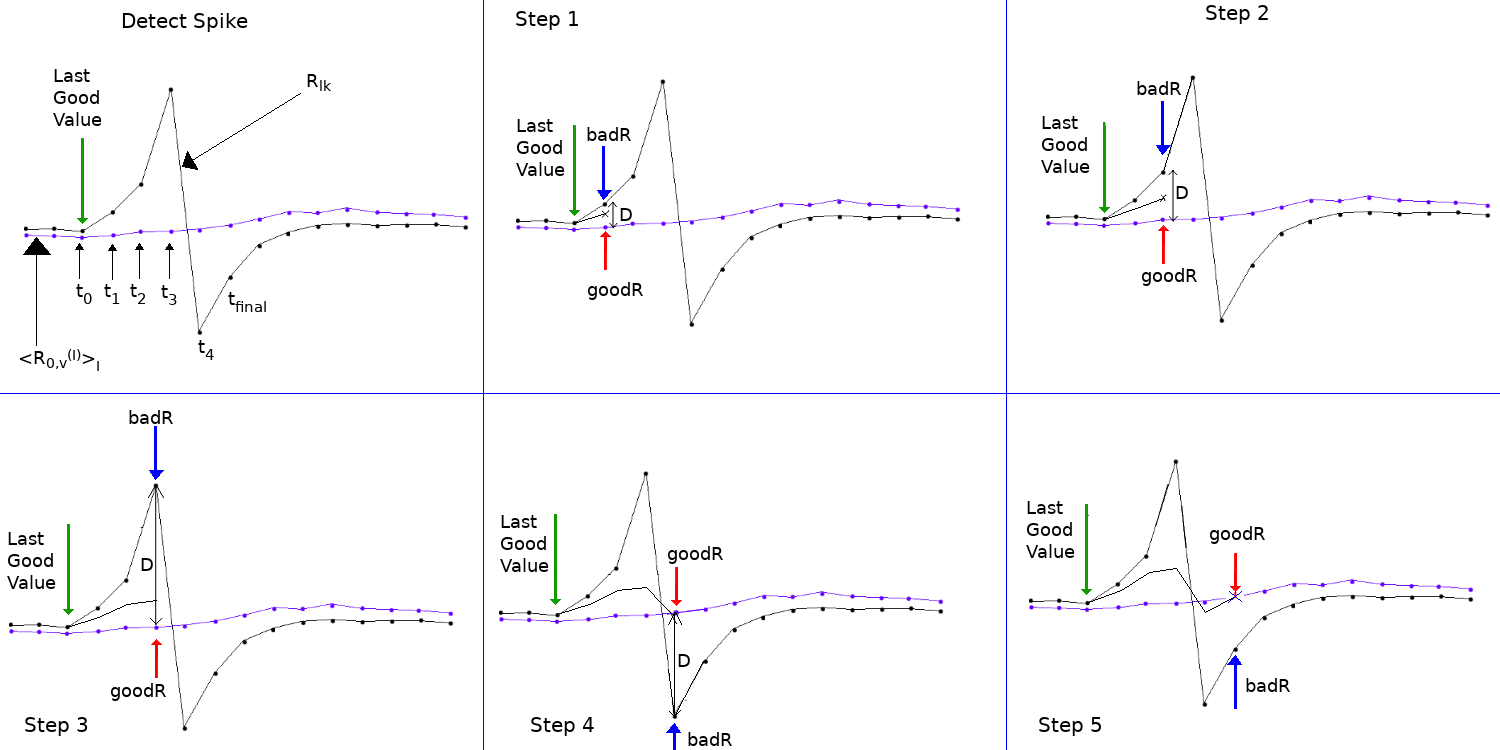
\includegraphics[width=\textwidth]{./img/CTMQC/tanh_explanation.png}
	\caption{\label{fig:tanh_explan}A crude demonstration of the principle behind the smoothing procedure in switching between intercepts. The black line shows an intercept begin to diverge and the alternative intercept is shown in purple. As the step is incremented the amount of the alternative intercept that makes up the effective intercept is increased until only 1 intercept is used.}
\end{figure}


\chapter{Rabi Oscillation \label{ap:Rabi}}
The time dependant Schr\"odinger equation is given below:
\begin{equation}
	i \hbar \frac{\delta}{\delta t} \Phi(\textbf{R}(t), t) = \hat{H}(\textbf{R}(t), t) \Phi(\textbf{R}(t), t)
\end{equation}
If we hold the nuclear coordinates in place (e.g. remove time-dependence from nuclear coordinates) we get an ordinary differential equation as shown below:
\begin{equation}
	i \hbar \frac{d}{d t} \Phi(\mathbf{R}, t) = \hat{H}(\mathbf{R}, t) \Phi(\mathbf{R}, t)
\end{equation}
This has the following general solution.
\[\Phi(\mathbf{R}, t) = e^{i \hbar \hat{H}t} \Phi(\mathbf{R}, 0)\]









\chapter{Norm Conservation in CTMQC and Ehrenfest}
\label{ap:norm_cons}
A statement of the conservation of the norm, for a single trajectory, is given below in equation \eqref{eq:normConsState}
\begin{equation}
	\frac{d}{dt} \sum_{l} \left\vert C_{l}(t) \right\vert^2 = \sum_{l} C_{l}^{*}(t)\frac{d C_{l}(t)}{dt} + \frac{d C_{l}^{*}(t)}{dt}C_{l}(t)
	\label{eq:normConsState} = 0
\end{equation}
Because the adiabatic populations are real we can remove any imaginary parts.
\begin{equation}
	\frac{d}{dt} \sum_{l} \left\vert C_{l}(t) \right\vert^2 = 2 \mathbb{R} \left[ C_{l}^{*}(t) \frac{d C_{l}(t)}{dt} \right]
	\label{eq:RealNorm}
\end{equation}
Substituting the equation for the evolution of the adiabatic coefficients (and removing the purely imaginary term) into \eqref{eq:RealNorm} we get equation \eqref{eq:KsumKadNorm}
\begin{align}
	\frac{d}{dt} \sum_{l} \left\vert C_{l}(t) \right\vert^2 &= 2 \sum_{l} \mathbb{R} \left[ \cancel{\frac{-i}{\hbar} \epsilon_{BO}^{l} C_l(t)^*C_l^{}(t)}
	- \sum_{k} \left[ C_l(t)^*C_k(t) d_{lk}^{ad} - (A_l - B_{l}) C_l(t)^*C_l(t)  \right] \right]
	\\
	&= -2 \sum_{l} \mathbb{R} \left[ \sum_{k} \left[ C_l(t)^*C_k(t) d_{lk}^{ad} - (A_l - B_{l}) C_l(t)^*C_l(t)  \right] \right]
	\label{eq:KsumKadNorm}
\end{align}
Where:
\begin{align}
	A_{l} &= \sum_{\nu = 1}^{N_n} \sum_{k} \frac{\mathcal{Q}_{lk, \nu}(t)}{\hbar M_\nu}\cdot \mathbf{f}_{k, \nu}(t) \vert C_k(t) \vert^2 \ \\
	B_{l} &= \sum_{\nu = 1}^{N_n} \sum_{k} \frac{\mathcal{Q}_{lk, \nu}(t)}{\hbar M_\nu}\cdot \mathbf{f}_{l, \nu}(t) \vert C_{k}(t)\vert^2
\end{align}
The NACE term evaluates to 0 due to the anti-symmetry of the NACE giving us equation \eqref{eq:KsumKadFinalNorm}. 
\\\\
So far, we have proved that the norm should be conserved here for all terms apart from the quantum momentum terms i.e. Ehrenfest.
\begin{align}
	\frac{d}{dt} \sum_{l} \left\vert C^{QM}_{l}(t) \right\vert^2 &= 2 \sum_{l} \mathbb{R} \left[ (A_l - B_{l}) C_l(t)^*C_l(t)  \right] \\
	&= 2 \left[ \sum_l A_l |C_{l}(t)|^2 - \sum_{l} B_{l} \vert C_{l}(t) \vert^2 \right]
	\label{eq:KsumKadFinalNorm}
\end{align}
However, $\sum_{l}A_l |C_{l}|^2 \equiv \sum_{l} B_{l} |C_{l}|^2$, therefore there is no change in the population and the norm should be conserved.
\newpage
\chapter{Adiabatic State Initialisation}
\label{ap:AdiabaticSelector}
By diagonalising the Hamiltonian we get the adiabatic energies (eigenvalues) for each state and transformation matrix (eigenvectors) to calculate diabatic states $\mathbb{U}$. We can calculate diabatic coefficients corresponding to each adiabatic state via equation \eqref{eq:CtoU_trans} below.
\begin{equation}
	\mathbb{U} \mathbf{C}_{n} = \mathbf{u}_{n}
	\label{eq:CtoU_trans}
\end{equation}
Where $\mathbb{U}$ is the transformation matrix of size (N$_{\text{mol}}$,  N$_{\text{mol}}$), $\mathbf{C}$ is a complex vector of size N$_{\text{mol}}$ containing coefficients for adiabatic state n and $\mathbf{u}$ is a complex vector of size N$_{\text{mol}}$ containing coefficients for diabatic state n.
\\\\
Seeing as we would like to find the diabatic population corresponding to each adiabatic state we localise coefficients on each pure adiabatic state and carry out the transformation e.g: $C_i = (1+0i, 0+0i, 0+0i, ...)$ when we want to find the diabatic coefficient corresponding to state 1 and $C_i = (0+0i, 1+0i, 0+0i, ...     )$ when we want to find the diabatic coefficient corresponding to state 2 etc.. Therefore, the column, n, of the transformation matrix, $\mathbb{U}$, gives the diabatic coefficients corresponding to adiabatic state, n, as shown below in equation \eqref{eq:trans_equal_u}
\begin{equation}
	U_{in} = u_{i}
	\label{eq:trans_equal_u}
\end{equation}
Where n is the adiabatic state index and i is the diabatic (molecular) state index.
\\\\
Once we have the diabatic state corresponding to each adiabatic state, and the energy of that adiabatic state, we can find which state best fulfills the requirements of being close to the center of the system and being within 3KT of the ground state. In order to do this, we can loop over each adiabatic state in increasing order of energy. The center of the system is calculated and the population weighted average center of mass, $\mathbf{R}_n$ of the diabatic coefficients corresponding to adiabatic state n is calculated as in equation \eqref{eq:COM_pop}.
\begin{equation}
	\mathbf{R}_{n} = \sum_{i} |u_{i}|^2 \mathbf{R}_{COM, i}
	\label{eq:COM_pop}
\end{equation}
The Euclidean distance between the center of the system and $\mathbf{R}_{COM, i}$ is calculated and if this distance is below some threshold value then we initialise the surface hopping trajectory on that adiabatic state. If we do not find any states within 3KT of the ground state and within an acceptable radius of the center we start again this time increasing the maximum allowed distance from the center. If this maximum allowed distance is increased such that we reach another threshold distance the energy threshold is increased this time until a state is found that is close enough to the center. In this way we find an adiabatic state, which when transformed, gives a diabatic population close to center of the system and near the ground state energy.



\chapter{Colophon}
\label{appendixlabel3}
\textit{This is a description of the tools you used to make your thesis. It helps people make future documents, reminds you, and looks good.}

\textit{(example)} This document was set in the Times Roman typeface using \LaTeX (specifically LuaTeX) and Bib\TeX , composed with Vim 
Used Archer, Kathleen etc...
 % description of document, e.g. type faces, TeX used, TeXmaker, packages and things used for figures. Like a computational details section.
% e.g. http://tex.stackexchange.com/questions/63468/what-is-best-way-to-mention-that-a-document-has-been-typeset-with-tex#63503

% Side note:
%http://tex.stackexchange.com/questions/1319/showcase-of-beautiful-typography-done-in-tex-friends
